\section{Additional Research}
In this section will discuss any extra research done on the project.
in this section we will discuss the following:
\begin{enumerate}
    \item ADC
    \item Radio module
\end{enumerate}
\subsection{ADC}
The MCP3008 was not  available when ordering parts,Another  part for this was choosen which is the  DFR0553 which has the following:
\begin{enumerate}
    \item a supply voltages(VCC) of 3.3 to 5 v
    \item Analog signal  detection 0 to 5v
    \item 4 analog chanel's
    \item resolution of 16 bits
    \item Operating current of 3mA
\end{enumerate}
\subsection{Radio module}
for  this  section we want  to keep  the following in mind :
\begin{enumerate}
    \item We want a module that will send  and  received data
    \item we don't  want  an  expensive solution due  to wanting to  have  multiple nodes
    \item must we pick a standard? 
    \item what module has  an open source project on it 
    \item how do we  set up  a   mesh network with this 
\end{enumerate}
\subsubsection{Do we need a radio standard?}
Lets assume we communicate with two pi via wires  we know that an interference will occur when  we  commutation that is wireless
we can have multiple cases where interference can  occur these are  the following:
\begin{enumerate}
    \item the signal being reflected of objects such as  trees
    \item the signal can reach the  receiver due to an object blocking the antenna
    \item the signal isn't  power to be picked up by the receiver
\end{enumerate}
one essential part of this project is the  ability to have  our nodes have an address to set this up
from a communication preceptive we could develop this when there is open source project that has sorted out the routeing for  you.
only issue with this approach is if there is any issues that come from the open source project we will inherit the bugs
with this in mind the following standards were found
\newpage
\begin{enumerate}
    \item LoRa
\end{enumerate}
\subsubsection{LoRa}

In \cite{Wu_Liebeherr_2023} lora is used that will organize sensor
data from all nodes in the spanning tree toward the root(laptop /PC) this can be show by the  following:
\begin{figure}[h!]
    \centering
    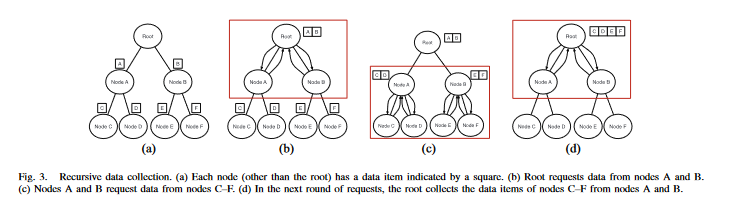
\includegraphics[width=0.5\linewidth]{Images/lora_example_routing_proto.png}
    \caption{protocol Wu used(wu\_lie et.al,2023:16705)}
    \label{protocol Wu used(wu_lie et.al,2023:16705)}
\end{figure}  
this proves it possible  to make a  mesh network using Lora.
\par 
from looking online Lora has more projects that are open source meaning we can use it.freely for example 
\par
Lora is uses spread spectrum modulation, In \cite{2003_Information_2023} spread spectrum is apparent in Shannon's theorem which states the channel capacity C the upper limit on the information rate of data that can be communciated at a lower error rate through the received signal power S:
$$C=B\log_2(1+\frac{S}{N})$$
Where B is the is the bandwidth of the channel in hertz.Where the bandwidth is:
$$B=F_{max}-F_{min}$$
spread spectrum  creates a pseudo-random code sequence that modulates the data signal  which will determine the  how  the signal is  spread out.

To simulate the system we can use the following FIR response  as an example 
\begin{figure}[h!]
    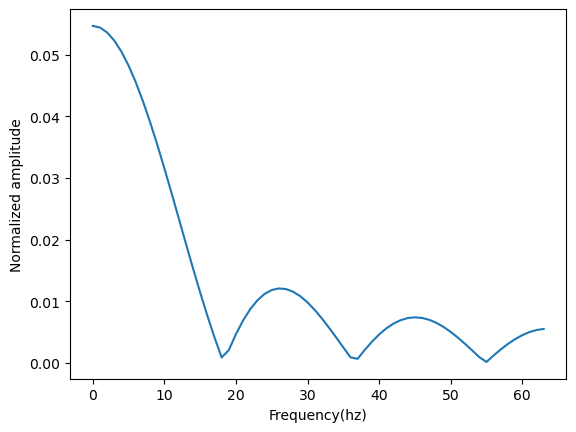
\includegraphics[width=0.5\linewidth]{Images/FIR_response.png}
    \caption{sample graph of a FIR response}
    \label{sample graph of a FIR response}

\end{figure}
in a given  medium  of  transmit each bandwidth is the length the of the  sinc-roll-off which degrade depends on the  impulse response in this given bandwidth channels are separated in the same fashion .
\subsection{What is  the difference  between a  port and a channel}
In \cite{flare} "A port is a virtual point where network connections start and end. Ports are software-based and managed by a computer's operating system. Each port is associated with a specific process or service. Ports allow computers to easily differentiate between different kinds of traffic: emails go to a different port than webpages, for instance, even though both reach a computer over the same Internet connection."
\newpage
\subsection{Why the MM2 Series 900 MHz wasn't picked}
When ordering the parts for  this module issues where due to company not selling the product to  enterprise-level businesses so then two alternative radio modules were found:
\begin{enumerate}
    \item SB Components LoRa HAT for Raspberry Pi
    \item RPIZ SHD LORA433 Raspberry Pi Shield - LoRa, 433 MHz, SX1268
\end{enumerate}
when we compare these we get the following table:

\begin{table}[h!]
    \scalebox{0.45}{
        \begin{tabular}{|l|l|l|l|l|l|l|l|l|}
            \hline
            \rowcolor[HTML]{343434} 
            \multicolumn{1}{|c|}{\cellcolor[HTML]{343434}\textbf{Modules}} & \multicolumn{1}{c|}{\cellcolor[HTML]{343434}\textbf{Tx/RX Voltage}} & \multicolumn{1}{c|}{\cellcolor[HTML]{343434}\textbf{Frequency}} & \multicolumn{1}{c|}{\cellcolor[HTML]{343434}\textbf{Range}} & \multicolumn{1}{c|}{\cellcolor[HTML]{343434}\textbf{TX/RX power}} & \multicolumn{1}{c|}{\cellcolor[HTML]{343434}\textbf{Through put}} & \multicolumn{1}{c|}{\cellcolor[HTML]{343434}\textbf{Error detection}} & \multicolumn{1}{c|}{\cellcolor[HTML]{343434}\textbf{Rx sensitivity}} & \multicolumn{1}{c|}{\cellcolor[HTML]{343434}\textbf{Hopping channel}} \\ \hline
            SX1268 433M LoRa HAT & 5v & \begin{tabular}[c]{@{}l@{}}410.125$\sim$493.125MHz \\ or \\ 850.125$\sim$930.125MHz\end{tabular} & \begin{tabular}[c]{@{}l@{}}5KM(Sunny day; open area;\\  Antenna: AUX 5dBi,\\  Height 2.5m; \\ Air Speed: 2.4kbps)\end{tabular} & 11ma /100ma & 0.3Kbps & None & -147dBm@0.3Kbps (On air) & None \\ \hline
            SB Components LoRa HAT for Raspberry Pi & 5v & 915/868/433 MHz & 5km & 22dBm & 0.3Kbps & None & N/A & None \\ \hline
            \end{tabular}        
        }
        \caption{Comparing New Radio modules}
        \label{Comparing New Radio modules}
\end{table}

\subsection{SB Components LoRa HAT}
Which has a  E22-900T22S on the  board which has a throughput rate of 0.3kbps\~62.5kbps so the maximum time it will take to get to a  node will be around 16 seconds depending on distance ,the module has two was of interacting with the board:
\begin{enumerate}
    \item Pi
    \item usb to windows desktop in this configuration we  can test single node from our laptop this is just to  test sending message across the serial 
\end{enumerate}
This hat supports three frequencies:
\begin{enumerate}
    \item 868 Mhz
    \item 433 Mhz
    \item 915 Mhz
\end{enumerate}
\subsubsection{E22-900T22S}
E22-900T22S is a wireless serial port module (UART) based on SEMTECH's SX1262 RF chip. It has multiple transmission modes, working in the 850.125MHz~930.125MHz, (default 900.125MHz).which has the following functions:
\begin{enumerate}
    \item LoRa spread spectrum
    \item Listen before talk(LBT):
    
    The module will monitor the channel  before transmitting data , if the environment exceeds the threshold. it will be delayed .
    \item RSSI(Received Signal Strength Indicator):
    \item Networking function: 
    \item Ultra-low power consumption
    \item Broadcast monitoring
\end{enumerate}